\documentclass[12pt]{article}
\usepackage[utf8]{inputenc}
\usepackage{amsmath}
\usepackage{amssymb}
\usepackage{amsthm}
\usepackage{fullpage}
\setlength\parindent{0pt}
\setlength{\parskip}{1em}
\newtheorem{theorem}{Theorem}[section]
\usepackage{tikz}
\usetikzlibrary{arrows,matrix,positioning}

\begin{document}

\begin{center}
    Linear Statistical Models - MAST30025 \\
    Akira Wang
\end{center}

\section{Linear Algebra Review}

\subsection{Transposition:}  
The \textit{transpose} of a matrix results when the rows and columns are interchanged. 

A matrix $X$ is \textbf{symmetric} if and only if (iff) $X^T = X$.

\fbox{
  \parbox{\textwidth}{
    Properties that should be noted:\\
    \begin{enumerate}  
        \item $(X^T)X = X$.
        \item $(XY)^T = Y^TX^T$.
    \end{enumerate}
  }
}

\subsection{Identity:}

The matrix \textit{identity $I$} is a square matrix of arbitrary size with 1's on the diagonals (diags).

A $k\times k$ identity matrix is denoted as $I_k$.

\subsection{Inverse:}

If $X$ is a \textbf{square matrix}, its \textit{inverse} is the matrix $X^{-1}$ of the same size which satisfies the following:

\begin{equation}
    XX^{-1} = X^{-1}X = I
\end{equation}

\fbox{
  \parbox{\textwidth}{
    Properties that should be noted:\\
    \begin{enumerate}  
        \item $(X^{-1})^{-1} = X$.
        \item $(XY)^{-1} = Y^{-1}X^{-1}$.
        \item $(X^T)^{-1} = (X^{-1})^T$
    \end{enumerate}
  }
}

\subsection{Orthogonal Vectors and Matrices:}
Two $n\times 1$ vectors $\mathbf{x}$ and $\mathbf{y}$ are \textit{orthogonal} iff:

\begin{equation}
    \mathbf{x}^T\mathbf{y} = \sum^{n}_{i=1}x_iy_i = 0.
\end{equation}

A square matrix $X$ is \textit{orthogonal} iff:

\begin{equation}
    X^TX = I.
\end{equation}

If X is orthogonal, then

\begin{equation}
    X^{-1} = X^T.
\end{equation}

\subsection{Orthogonality:}

\begin{equation}
    \textrm{If } \mathbf{x} = \begin{bmatrix} x_1 \\ x_2 \\ \vdots \\ x_n \end{bmatrix}\textrm{, then }\mathbf{x}^T\mathbf{x} = ||\mathbf{x}||^2 = \sum^n_{i=1}x^2_i
\end{equation}

The square root of $||\mathbf{x}^2||$, denoted by $||\mathbf{x}||$, is called the \textbf{norm} or \textbf{length} of \mathbf{x}.

A matrix $X$ is an orthogonal matrix iff the columns of $X$ form an orthonormal set.

\subsection{Eigenvalues and Eigenvectors:}

Suppose $A$ is a $k\times k$ matrix and \mathbf{x} is a $k\times 1$ nonzero vector which satisfies the equation

\begin{equation}
    A\mathbf{x} = \lambda\mathbf{x}.
\end{equation}

We say that $\lambda$ is an \textit{eigenvalue} of $A$, with associated \textit{eigenvector} $\mathbf{x}$.

To find the eigenvalues, solve the following equation:

\begin{equation}
    |A - \lambda I| = 0.
\end{equation}

To then find the eigenvector(s) of $A$ associated with the eigenvalue(s), solve the linear system of equations:

\begin{equation}
    A\mathbf{x} = \lambda\mathbf{x}.
\end{equation}

The linear system should have an infinite number of solutions, which will always happen for an eigenvector system.

\fbox{
  \parbox{\textwidth}{
    Note:\\
    \begin{enumerate}  
        If $A$ is \textbf{symmetric}, then all its eigenvalues are \textbf{real}, and its eigenvectors all \textbf{orthogonal}.
    \end{enumerate}
  }
}

\subsection{Diagonalization:}

Let $A$ be a \textbf{symmetric} $k\times k$ ,matrix. Then an \textbf{orthogonal} matrix $P$ exists such that

\begin{equation}
    P^TAP = \begin{bmatrix} \lambda_1 & 0  & \dots  & 0 \\ 0 & \lambda_2  & \dots  & 0 \\ \vdots & \vdots & \vdots & \ddots \\ 0 & 0 & \dots & \lambda_k \end{bmatrix}\\
    \textrm{where }\lambda_i, i = 1, 2, \dots, k, \textrm{are the eigenvalues of } A.
\end{equation}

We say that $P$ \textit{diagonalizes} $A$, where $A$ is the \textit{diagonalizable} matrix, and $P^TAP$ is the \textit{diagonalized} matrix.

\subsection{Linear Independence:}
A set of vectors is \textit{linearly depending} iff there exists some numbers $\alpha_1, \alpha_2, \dots, \alpha_k$, which are not all zero, such that

\begin{equation}
    \alpha_1\mathbf{x}_1  +  \alpha_2\mathbf{x}_2 +  \alpha_k\mathbf{x}_k = \mathbf{0}.
\end{equation}

If all $\alpha$ are zero, then they are are \textit{linearly independent}.

If a set of vectors is linearly dependent, then at least one of the vectors can be written as a \textbf{linear combination} of some or all the other vectors.

\subsection{Rank:}

\fbox{
  \parbox{\textwidth}{
    Some definitions (Yao-Ban):\\
    \begin{enumerate}  
        \item Tall Matrix has more rows than columns ($m>n$) and is of \textit{\textbf{full rank}}.
        \item Short Matrix has more columns than rows ($n>m$).
    \end{enumerate}
  }
}

The \textit{rank} of $X$, denoted by $r(X)$, is the greatest number of \textbf{linearly independent vectors} in the set $\left\{\mathbf{x}_1, \mathbf{x}_2, \dots, \mathbf{x}_k\right\}$.

\fbox{
  \parbox{\textwidth}{
    Properties that should be noted:\\
    \begin{enumerate}  
        \item For any matrix $X$, we have $r(X) = r(X^T) = r(X^TX)$
        \item The rank of a diagonal matrix is equal to the number of nonzero diagonal entries in the matrix.
    \end{enumerate}
  }
}

\subsection{Idempotence:}

A square matrix $A$ is \textit{idempotent} iff

\begin{equation}
    A^2=A
\end{equation}

It should be noted that if $A$ is diagonizable, then $A$ is idempotent.

\fbox{
  \parbox{\textwidth}{
    Properties that should be noted:\\
    \begin{enumerate}  
        \item The eigenvalues of any idempotent matrix is always either $0$ or $1$\\
        \textbf{Proof.}\\
        
        \begin{*align}
            A^2\mathbf{x} &= A(A\matbf{x})\\
                          &= A(\lambda\matbf{x}), \textrm{since } A\mathbf{x} = \lambda\mathbf{x}\\
                          &= \lambda (A\mathbf{x})\\
                          &= \lambda^2\mathbf{x}\\\\
        \end{*align}
        By definition, $\mathbf{x} \neq \mathbf{0}$, so $\lambda = \lambda^2$. Therefore $\lambda = 0, 1$.
        
        \item If $A$ is a \textbf{symmetric} and \textbf{idempotent} matrx, $r(A) = tr(A)$.
        
    \end{enumerate}
  }
}

\subsection{Trace:}

The \textit{trace} of a square matrix $X$, denoted by $tr(X)$, is the sum of its diagonal entries

\begin{equation}
    tr(X) = \sum^{k}_{i=1}x_{ii}.
\end{equation}

\fbox{
  \parbox{\textwidth}{
    Properties that should be noted:\\
    \begin{enumerate}  
        \item If $c$ is a scalar, $tr(cX) = c tr(X)$
        \item If $XY$ and $YX$ both exist, $tr(XY) = tr(YX)$
    \end{enumerate}
  }
}

\subsection{Quadratic Forms:}

Suppose $A$ is a square matrix, and \mathbf{y} is a $k\times 1$ vector containing variables. The quantity

\begin{equation}
    q = \mathbf{y}^TA\mathbf{y}
\end{equation}

is called a \textit{quadratic form} in $\mathbf{y}$, and $A$ is called the matrix of the \textit{quadratic form}.

However, since $q$ is a scalar, it can be re-expressed as

\begin{equation}
    q = \sum^{k}_{i=1}\sum^{k}_{j=1}a_{ij}y_iy_j.
\end{equation}

\textbf{Example:}\\

\[\textrm{Let }\mathbf{y} = \begin{bmatrix} y_1 \\ y_2 \\ y_3 \end{bmatrix}, \textrm{and } A=
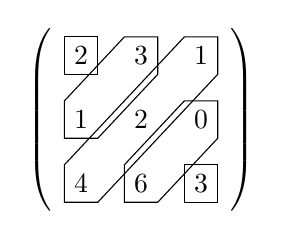
\begin{tikzpicture}[baseline=-\the\dimexpr\fontdimen22\textfont2\relax ]
        \matrix [matrix of math nodes,row sep=10pt,column sep = 10pt,left delimiter=(,right delimiter=)] (m)
        {
            2 &3 &1 \\               
            1 &2 &0 \\               
            4 &6 &3 \\           
        };  
        \draw (m-1-2.north west) -- (m-2-1.north west) -- (m-2-1.south west) -- (m-2-1.south east) -- (m-1-2.south east) -- (m-1-2.north east) -- cycle;
        \draw (m-1-1.north west) -- (m-1-1.south west) -- (m-1-1.south east) -- (m-1-1.north east) -- cycle;
        \draw (m-1-3.north west) -- (m-3-1.north west) -- (m-3-1.south west) -- (m-3-1.south east) -- (m-1-3.south east) -- (m-1-3.north east) -- cycle;
        \draw (m-2-3.north west) -- (m-3-2.north west) -- (m-3-2.south west) -- (m-3-2.south east) -- (m-2-3.south east) -- (m-2-3.north east) -- cycle;
        \draw (m-3-3.north west) -- (m-3-3.south west) -- (m-3-3.south east) -- (m-3-3.north east) -- cycle;
\end{tikzpicture}
\]

Then

\begin{align}
    \mathbf{y}^TA\mathbf{y} &= \Bigm|2y^2_1\Bigm| + \Bigm|3y_1y_2 + y_1y_3\Bigm| + \Bigm|y_2y_1 + 2y^2_2 + 4y_3y_1\Bigm| + \Bigm|0 + 6y_3y_2\Bigm| + \Bigm|3y^2_3\Bigm|\\
                            &= 2y^2_1 + 2y^2_2 + 3y^2_3 + 4y_1y_2 + 5y_1y_3 + 6y_2y_3
\end{align}

This can be found from either the summation formula (14) or by multiplying out the matrices.

\fbox{
  \parbox{\textwidth}{
    Positive Definiteness:\\
    \begin{enumerate}  
        \item If $\mathbf{y}^TA\mathbf{y} > 0$, then it is \mathbf{\mathit{positive definite}}.
        \item If $\mathbf{y}^TA\mathbf{y} \geq 0$, then it is \mathbf{\mathit{positive semi-definite}}.
    \end{enumerate}
  }
}

\fbox{
  \parbox{\textwidth}{
    Properties that should be noted:\\
    \begin{enumerate}  
        \item The quadratic form will \textbf{never} be negative.
        \item A symmetric matrix $A$ is \textbf{positive definite} iff all its eigenvalues are all (strictly) positive.
        \item A symmetric matrix $A$ is \textbf{positive semi-definite} iff all its eigenvalues are all non-negative.
    \end{enumerate}
  }
}

\subsection{Differentiation of Quadratic Forms:}

Suppose we have a vector of variables $\mathbf{y} = (y_1,y_2,\dots,y_k)^T$, and some scalar function of them

\begin{equation}
    z = f(\mathbf{y}).
\end{equation}

We can then define the derivative of $z$ with respect to $\mathbf{y}$ as follows:

\begin{equation}
    \frac{\partial z}{\partial\mathbf{y}} = \begin{bmatrix} \frac{\partial z}{\partial y_1} \\ \frac{\partial z}{\partial y_2} \\ \vdots \\ \frac{\partial z}{\partial y_k} \end{bmatrix}
\end{equation}

To do so, you can take the \textbf{quadratic form} of $z$ and \textbf{partial derive} with respect to $\mathbf{y}.$

\textbf{Example from Figure 14:}\\

\begin{equation}
    \frac{\partial z}{\partial\mathbf{y}} = \begin{bmatrix} 4y_1 + 4y_2 + 5y_3 \\ 4y_2 + 4y_1 + 6y_3 \\ 6y_3 + 5y_1 + 6y_2 \end{bmatrix}
\end{equation}

\section{Random Vectors}

\subsection{Expectation:}

\textbf{Note that we will denote random variables (r.v's) as lower-cases, according to linear algebra notation.}

We define the \textit{expectation} of a random vector $\mathbf{y}$ as follows:

\begin{equation}
    \textrm{If }\mathbf{y} = \begin{bmatrix} y_1 \\ y_2 \\ \vdots \\ y_k \end{bmatrix},\textrm{then } E[\mathbf{y}] = \begin{bmatrix} E[y_1] \\ E[y_2] \\ \vdots \\ E[y_k] \end{bmatrix}
\end{equation}

\fbox{
  \parbox{\textwidth}{
    Properties that should be noted:\\
    \begin{enumerate}  
        \item If $\mathbf{a}$ is a vector of constants, then:
        \begin{enumerate}
            \item $E[\mathbf{a}] = \mathbf{a}.$
            \item $E[\mathbf{a}^T\mathbf{y}] = \mathbf{a}^Te[\mathbf{a}].$
        \end{enumerate}
        \item If $A$ is a matrix of constants, then $E[A\mathbf{y}] = AE[$\mathbf{y}].
    \end{enumerate}
  }
}

\subsection{Variance:}







\end{document}





